%%%%%%%%%%%%%%%%%%%%%%%%%%%%%%%%%%%%%%%%%%%%%%%%%%%%%%%%%%%%%%%%%%%%%%%%%%%%%%%%%%%%%%%%%%%%%%%%%%%%%%%%%%%%%%%%%%%%%%
\chapter{Results for non separable $p$} \label{sec:para}%%%%%%%%%%%%%%%%%%%%%%%%%%%%%%%%%%%%%%%%%%%%%%%%%%%%%%%%%%%%%%
%%%%%%%%%%%%%%%%%%%%%%%%%%%%%%%%%%%%%%%%%%%%%%%%%%%%%%%%%%%%%%%%%%%%%%%%%%%%%%%%%%%%%%%%%%%%%%%%%%%%%%%%%%%%%%%%%%%%%%
We start by showing convergence in section \ref{sec:pconv}, and proceed with looking into speedup and parallel efficiency in section \ref{sec:speed}. We end by investigating how computation time for the best possible case of KPM compares to DM. 

%%%%%%%%%%%%%%%%%%%%%%%%%%%%%%%%%%%%%%%%%%%%%%%%%%%%%%%%%%%%%%%%%%%%%%%%%%%%%%%%%%%%%%%%%%%%%%%%%%%%%%%%%%%%%%%%%%%%%%
\section{Convergence} \label{sec:pconv}
%%%%%%%%%%%%%%%%%%%%%%%%%%%%%%%%%%%%%%%%%%%%%%%%%%%%%%%%%%%%%%%%%%%%%%%%%%%%%%%%%%%%%%%%%%%%%%%%%%%%%%%%%%%%%%%%%%%%%%
\begin{figure}[H]
        \centering
        \begin{subfigure}[b]{0.45\textwidth}
                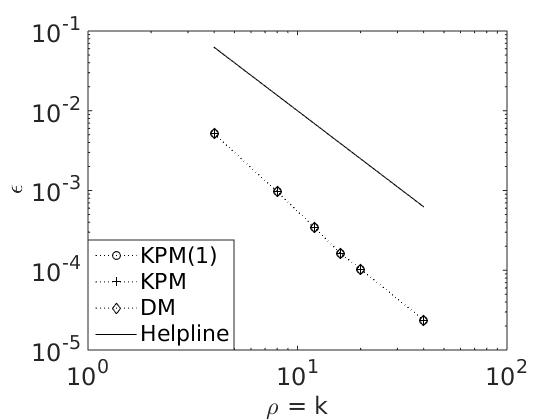
\includegraphics[width=\textwidth]{fig/p1conv1}
                %\includegraphics[width=\textwidth]{test}
                \caption{function \texttt{P1}}
                \label{fig:conv1p}
        \end{subfigure}%
        ~
        \begin{subfigure}[b]{0.45\textwidth}
                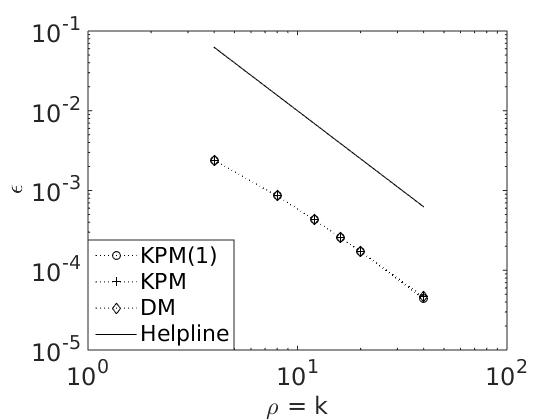
\includegraphics[width=\textwidth]{fig/p2conv2}
                %\includegraphics[width=\textwidth]{test}
                \caption{function \texttt{P3}}
                \label{fig:conv2p}
        \end{subfigure}
        \caption{A convergence plot for several method with $\rho = k$. The helpline shows quadratic convergence.}\label{fig:convp}
\end{figure}
As can be seen from figure \ref{fig:convp}, all methods converges quadratically and identically, as in the serial case. 
%%%%%%%%%%%%%%%%%%%%%%%%%%%%%%%%%%%%%%%%%%%%%%%%%%%%%%%%%%%%%%%%%%%%%%%%%%%%%%%%%%%%%%%%%%%%%%%%%%%%%%%%%%%%%%%%%%%%%%
\section{Speedup} \label{sec:speed}
%%%%%%%%%%%%%%%%%%%%%%%%%%%%%%%%%%%%%%%%%%%%%%%%%%%%%%%%%%%%%%%%%%%%%%%%%%%%%%%%%%%%%%%%%%%%%%%%%%%%%%%%%%%%%%%%%%%%%%
\begin{figure}[H]
        \centering
        \begin{subfigure}[b]{0.45\textwidth}
                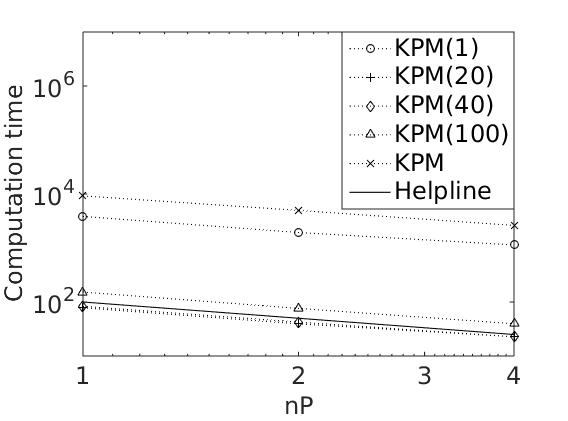
\includegraphics[width=\textwidth]{fig/u1para1}
                %\includegraphics[width=\textwidth]{test}
                \caption{function \texttt{P1}}
                \label{fig:speed1}
        \end{subfigure}%
        ~
        \begin{subfigure}[b]{0.45\textwidth}
                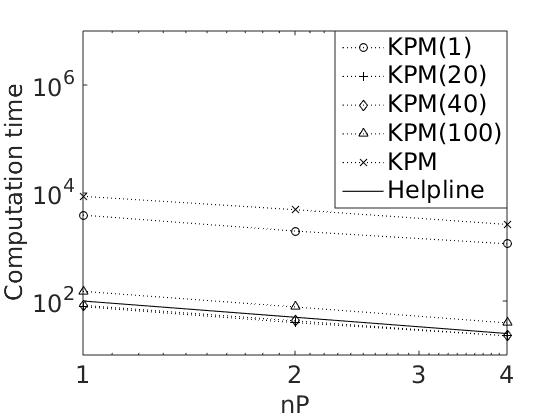
\includegraphics[width=\textwidth]{fig/u2para2}
                %\includegraphics[width=\textwidth]{test}
                \caption{function \texttt{P3}}
                \label{fig:speed2}
        \end{subfigure}
        \caption{Computation times for several methods with different number of processors. The helpline shows perfect speedup.}\label{fig:speed}
        
\end{figure}

\begin{table}[H]
\centering
\begin{tabular}{l| l l | l l}
&\texttt{P1} & & \texttt{P3} & \\
&\texttt{nP = 2} & \texttt{nP = 4} & \texttt{nP = 2} & \texttt{nP = 4} \\
\hline
KPM & 1.8556  &  3.5234 & 1.7702&    3.3193\\
KPM$(1)$ & 1.9858  &  3.3740 & 1.9725&    3.3924\\
KPM$(20)$ & 1.9883  &  3.4525 & 1.9756&    3.4547\\
KPM$(40)$ & 1.9619  &  3.6667 & 1.9352&   3.6642\\
KPM$(100)$ & 2.0083  &  3.8618 & 1.9437&    3.8362\\
\end{tabular}
\caption{Speedup for several cases of KPM.}
\label{tab:speedup}
\end{table}

\begin{table}[H]
\centering
\begin{tabular}{l|l l| l l}
&\texttt{P1} & & \texttt{P3} & \\
&\texttt{nP = 2} & \texttt{nP = 4} & \texttt{nP = 2} & \texttt{nP = 4} \\
\hline
KPM & 0.9278  &  0.8809 & 0.8851&    0.8298\\
KPM$(1)$ &  0.9929  &  0.8435 & 0.9862 &   0.8481\\
KPM$(20)$ & 0.9942  &  0.8631 & 0.9878&    0.8637\\
KPM$(40)$ & 0.9809  &  0.9167 & 0.9676&    0.9160\\
KPM$(100)$ & 1.0042  &  0.9655 & 0.9719&    0.9591\\
\end{tabular}
\caption{Parallel efficiency for several cases of KPM. }
\label{tab:eff}
\end{table}
%!!!!!!!!!!!!!!!!!!!!!!!!!!IKKE FORNØYD MED DENNE!!!!!!!!!!!!!!!!!!\\
Figure \ref{fig:speed} shows good speedup for all methods. Table \ref{tab:speedup} and \ref{tab:eff} shows that KPM$(n)$ has almost perfect speedup. It is definitely efficient to use several processors on these types of problems. KPM and KPM$(1)$ is not as well suited for this, they probably uses to much memory or too many iterations to be efficient. The optimal value for $n$ with parallel computations seems to be to $n = 100$.
%%%%%%%%%%%%%%%%%%%%%%%%%%%%%%%%%%%%%%%%%%%%%%%%%%%%%%%%%%%%%%%%%%%%%%%%%%%%%%%%%%%%%%%%%%%%%%%%%%%%%%%%%%%%%%%%%%%%%%
\section{Comparison}
%%%%%%%%%%%%%%%%%%%%%%%%%%%%%%%%%%%%%%%%%%%%%%%%%%%%%%%%%%%%%%%%%%%%%%%%%%%%%%%%%%%%%%%%%%%%%%%%%%%%%%%%%%%%%%%%%%%%%%
\begin{figure}[H]
        \centering
        \begin{subfigure}[b]{0.45\textwidth}
                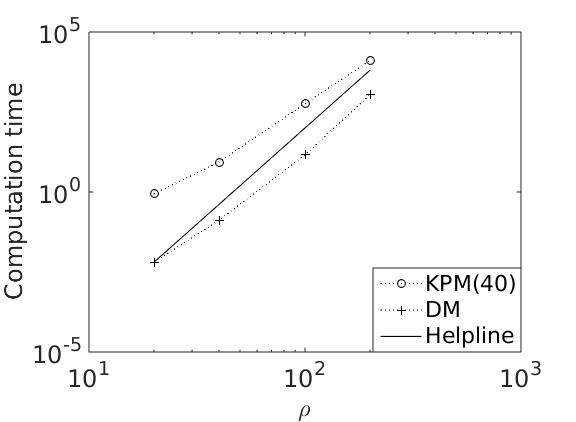
\includegraphics[width=\textwidth]{fig/c1comp1m}
                \caption{function \texttt{P1}}
                \label{fig:c1comp1m}
        \end{subfigure}%
        ~
        \begin{subfigure}[b]{0.45\textwidth}
                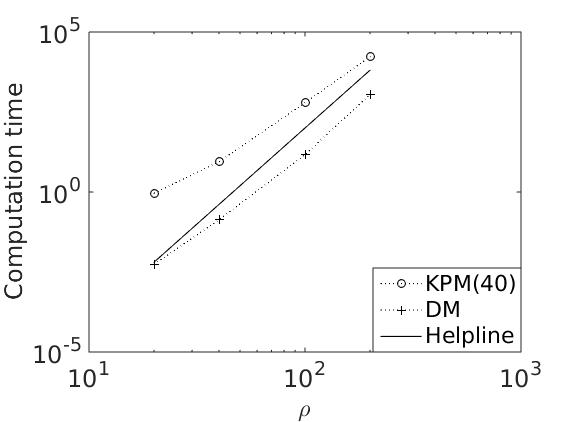
\includegraphics[width=\textwidth]{fig/c2comp2m}
                \caption{function \texttt{P3}}
                \label{fig:c2comp2m}
        \end{subfigure}
        
        \begin{subfigure}[b]{0.45\textwidth}
                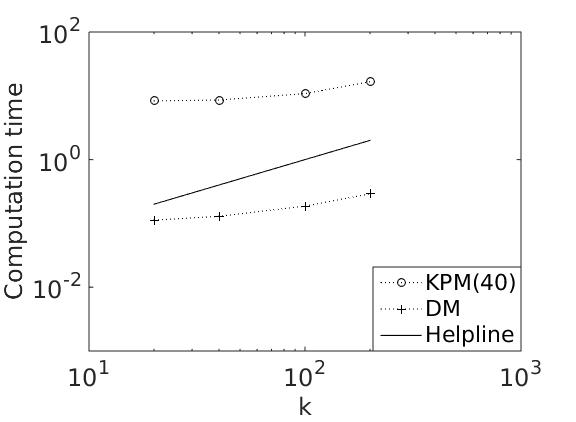
\includegraphics[width=\textwidth]{fig/c3comp1k}
                \caption{function \texttt{P1}}
                \label{fig:c3comp1k}
        \end{subfigure}%
        ~
        \begin{subfigure}[b]{0.45\textwidth}
                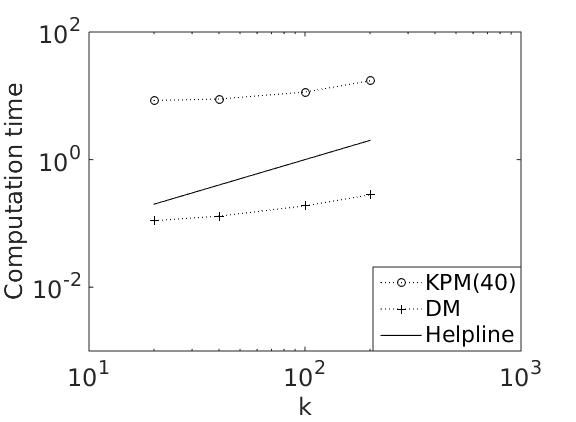
\includegraphics[width=\textwidth]{fig/c4comp2k}
                \caption{function \texttt{P3}}
                \label{fig:c4comp2k}
        \end{subfigure}
        \caption{A plot of the computation times tuned to be as efficient as possible for KPM$(n)$. Values are as follows: $n = \rho = k = 40$, $\delta = 10^{-4}$, $\texttt{nP} = 4$ when nothing else is stated. The helpline for figure \ref{fig:c1comp1m} and \ref{fig:c2comp2m} increases with $\rho^6 = m^3$, while the helpline for figure \ref{fig:c3comp1k} and \ref{fig:c4comp2k} increases with $k$.}\label{fig:comp}
        
\end{figure}
From figure \ref{fig:comp} it is clear that DM is better in all scenarios simulated here, but KPM$(n)$ is not far behind, with more processing units KPM$(40)$ could have been faster. The other important thing to note here is that computation time for KPM$(n)$ does not increase faster than for DM. It is difficult to say what would happen with larger $\rho$ or $k$, but they would probably follow the helpline.

One unfortunate simplification done is keeping $\delta$ constant while increasing $\rho$. This might not have a great impact in the result, but as shown in figure \ref{fig:errant} and \ref{fig:errtolk} it is of no use to increase $\rho$ and $k$ without decreasing $\delta$. It would also be of interest to increase $n$ while increasing $\rho$, as suggested by figure \ref{fig:rest}.